\section*{Acceptance page 78}
\label{page:78}
English text repeats: repeat repeat repeat. Editable word: alpha.
Chinese text: 中文排版测试，数学与文字同步。\par
Shared source line: $x+x+y=\frac{a_{1}+b^{2}}{c+d}+\alpha+\sum_{j=1}^{n}j$.
Nested math: $\frac{x+\frac{a}{b}}{y_{2}}$; macro argument: $\pair{z}$; generated macro: $\fixed$.
\begin{align*}
 f(x)&=x^{2}+2x+1\\
 g(x)&=\int_{0}^{1} t^{2}\,dt
\end{align*}
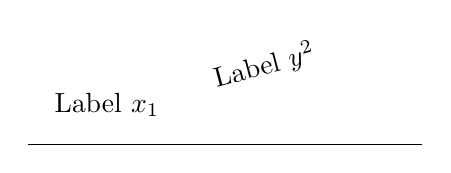
\begin{tikzpicture}
\draw (0,0) -- (5,0);
\node at (1,0.5) {Label $x_{1}$};
\node[rotate=15] at (3,1) {Label $y^{2}$};
\end{tikzpicture}
\par Cross-reference: page \pageref{page:1}. Macro: \globalword.
Paragraph 1: A stable reference sentence with repeated words and enough material to exercise paragraph layout. Changes to line breaking must preserve the complete-build result.\par
Paragraph 2: A stable reference sentence with repeated words and enough material to exercise paragraph layout. Changes to line breaking must preserve the complete-build result.\par
Paragraph 3: A stable reference sentence with repeated words and enough material to exercise paragraph layout. Changes to line breaking must preserve the complete-build result.\par
Paragraph 4: A stable reference sentence with repeated words and enough material to exercise paragraph layout. Changes to line breaking must preserve the complete-build result.\par
Paragraph 5: A stable reference sentence with repeated words and enough material to exercise paragraph layout. Changes to line breaking must preserve the complete-build result.\par
Paragraph 6: A stable reference sentence with repeated words and enough material to exercise paragraph layout. Changes to line breaking must preserve the complete-build result.\par
Paragraph 7: A stable reference sentence with repeated words and enough material to exercise paragraph layout. Changes to line breaking must preserve the complete-build result.\par
Paragraph 8: A stable reference sentence with repeated words and enough material to exercise paragraph layout. Changes to line breaking must preserve the complete-build result.\par
\newpage
